\label{chap:map}
A partir do levantamento dos diferentes tipos de avaliação, realizado no \refCap{chap:ref}, e da listagem das ferramentas, apresentada no \refCap{chap:ava}, propõe-se aqui uma estratégia de mapeamento de uma possível relação existente entre os tipos de avaliação com as ferramentas de AVA. Ou seja, cada tipo de avaliação pode ser relacionada a cada ferramenta da listagem \textbf{ (--> A QUE catálogo você se refere?)} \textcolor{blue} {corrigido} obtendo-se, ao final, uma matriz que represente essa relação. A \refFig{fig:passos} ilustra o processo de mapeamento proposto.
\\
\begin{figure}[h]
    \centering
\tikzset{
    mynode/.style={
        draw, rectangle, align=center, text width=5cm, font=\small, inner sep=1ex},
    mylabel/.style={
        draw, rectangle, align=center, rounded corners, font=\small\bf, inner sep=1ex, 
        fill=cyan!30, minimum height=2.5cm},
    arrow/.style={
        very thick,->,>=stealth}
}

\begin{tikzpicture}[
    node distance=1.5cm,
    start chain=1 going below,
    every join/.style=arrow,
    ]
    % the chain in the center going below
    \coordinate[on chain=1] (tc);
    \node[mynode, on chain=1] (n2)
        {Estabelecimento da relação\\entre (Y)x(W)};
    \node[mynode, join, on chain=1] (n3)
        {Estruturação do mapeamento em uma matriz de associação};

    % the nodes at the top  
    \node[mynode, left=1cm of tc, anchor=south east] (n1l)
        {Levantamento dos tipos\\ de avaliação (Y)};
    \node[mynode, right=1cm of tc, anchor=south west] (n1r) 
        {Listagem das ferramentas avaliativas (W)};

    \coordinate (n2nl) at ([xshift=-2cm]n2.north);
    \coordinate (n2nr) at ([xshift= 2cm]n2.north);
    \draw[arrow] (n1l.south -| n2nl) -- (n2nl);
    \draw[arrow] (n1r.south -| n2nr) -- (n2nr);

    % the labels on the left
    \begin{scope}[start chain=going below, xshift=-8cm, node distance=.8cm]
        \node[mylabel, on chain] {\rotatebox{90}{Identificação}};
        \node[mylabel, on chain] {\rotatebox{90}{Mapeamento}};
    \end{scope}

    % the title
    \node[above=1.5cm of tc, font=\bf] {Processo de Mapeamento};
\end{tikzpicture}
    \caption{Passos do mapeamento.}
    \label{fig:passos}
\end{figure}

%\textbf{--> NÃO PODES terminar uma seção com imagem. Tens que finalizar com um texto que faz um link com a seção seguinte.}
Essa proposta de mapeamento parte do pressuposto de que as ferramentas de um AVA são, em sua maioria, tentativas de representações virtuais de situações reais que aconteceriam em sala de aula. Portanto, cada uma delas pode representar também uma possibilidade de acompanhamento e de avaliação por parte do docente. A próxima seção tentará estabelecer essa relação.  
%%%%%%%%%%%%%%%%%%%%%%%%%%%%%%%%%%%%%%%%%%%%%%%%%%%
%%%%%%%%%%%%%%%%%%%%%%%%%%%%%%%%%%%%%%%%%%%%%%%%%%%
%%%%%%%%%%%%%%%%%%%%%%%%%%%%%%%%%%%%%%%%%%%%%%%%%%%
%%%%%%%%%%%%%%%%%%%%%%%%%%%%%%%%%%%%%%%%%%%%%%%%%%%

\section{Relação entre avaliação e ferramentas}

%Para estabelecer a relação entre uma ferramenta (W) e um tipo de avaliação (Y), houve a necessidade de se responder à seguinte pergunta: qual a potencial aplicabilidade da ferramenta na categoria de avaliação investigada?

A relação entre um tipo de avaliação (Y) e uma ferramenta (W), pode ser estabelecida de acordo com o objetivo que se deseja investigar. No escopo desse trabalho, por exemplo, o propósito é mapear se um dado tipo de avaliação pode ser aplicada por meio de uma determinada ferramenta. Sendo assim, a pergunta ``é aplicável?'' foi formulada para estabelecer essa relação entre (Y)x(W) que se deseja estudar. \textbf{(--> POR QUE TENS que responder a esta pergunta? Tens que explicitar isso)} \textcolor{blue} {alterado} As possíveis respostas para a pergunta foram parametrizadas conforme abaixo:

%Cabe ressaltar que podem haver outras relações entre esses elementos, com outros objetivos que não serão explorados aqui.
\begin{itemize}
    \item Aplicável, quando a definição da avaliação descreve propriamente o uso da funcionalidade da ferramenta, considerando-se suas características. O símbolo ``\ding{108}'' foi utilizado para representar graficamente a resposta.
    \item Parcialmente aplicável, quando a definição da avaliação descreve parte da funcionalidade. O símbolo ``\ding{115}'' representa a resposta. \item Não aplicável, quando a definição da avaliação não descreve o uso da funcionalidade. O símbolo ``\ding{53}'' representa a resposta. 
\end{itemize}

Considerando a relação e os parâmetros definidos, a ferramenta ``Acompanhar questionário'', do perfil do professor, poderia ser analisada, por exemplo, sob o aspecto da formalização da avaliação. Assim, ela pode ser classificada como \textbf{aplicável para a prática da avaliação formal}, já que atua com questionários que podem ser utilizados para aplicação de notas. E como \textbf{parcialmente aplicável na avaliação informal}, já que também fornece dados estatísticos ao docente sobre seu uso pelos alunos. A \refTab{tab:relYxW} utiliza a representação gráfica mencionada anteriormente para demonstrar a Relação (Y)x(W) da ferramenta ``Acompanhar questionário''.

\begin{table}[ht!]
\setlength{\bigstrutjot}{3pt}
\settowidth\rotheadsize{long text}
\caption{Relação (Y)x(W)}
\label{tab:relYxW}
\centering
\begin{tabular}{|l|c|c|}
\addlinespace \hline
    \bigstrut \textbf{Ferramentas do}  & \multicolumn{2}{c|}{Formalização}\\
\cline{2-3}
    \bigstrut
    \textbf{perfil professor}  & Formal & Informal \\
\hline
    \bigstrut[t]
    Acompanhar questionários & \ding{108} & \ding{115}\\ 
\hline
\end{tabular}
\end{table}

%\textbf{--> ESTE TRECHO está bastante confuso... Recomendo reescrever. Tens que fazer referência à imagem onde estao as ferramentas 3.4}
Do mesmo modo, a aplicabilidade de cada uma das ferramentas do perfil professor, apresentadas na \refFig{fig:ferramentas}, podem ser verificadas quanto ao aspecto da formalização. Os resultados completos para cada item da listagem são apresentados na \refTab{tab:tabrelYxW}.

\begin{table}[ht!]
\setlength{\bigstrutjot}{3pt}
\settowidth\rotheadsize{long text}
\caption{Lista da Relação (Y)x(W)}
\label{tab:tabrelYxW}
\centering
\begin{tabular}{|l|c|c|}
\addlinespace \hline
    \bigstrut \textbf{Ferramentas do}  & \multicolumn{2}{c|}{Formalização}\\
\cline{2-3}
    \bigstrut
    \textbf{perfil professor}  & Formal & Informal \\
\hline
    \bigstrut[t]
    Gerenciamento de grupo	& \ding{108} & \ding{115}\\ \hline
    Programação do curso    & \ding{108}  & \ding{53}\\ \hline
    Acompanhar anúncios     & \ding{53} & \ding{108}\\ \hline
    Acompanhar notificações & \ding{53} & \ding{108}\\ \hline
    Recuperação de conteúdo & \ding{53} & \ding{108}\\ \hline
    Map. de competências    & \ding{53} & \ding{108}\\ \hline
    Acompanhar colaboração  & \ding{115} & \ding{108}\\ \hline
    Acompanhar dificuldades & \ding{53} & \ding{108}\\ \hline
    Acompanhar questionários & \ding{108} & \ding{115}\\ \hline
    Revisão de textos       & \ding{108}  & \ding{53}\\ \hline 
    Acompanhar tarefas      & \ding{108}  & \ding{53}\\ \hline  
    Acompanhar aulas        & \ding{53} & \ding{108}\\ \hline
    Acompanhar exames       & \ding{108}  & \ding{53}\\ \hline  
    Registrar notas         & \ding{108}  & \ding{53}\\ \hline 
    Acompanhar notas/feedback  & \ding{53} & \ding{108}\\ \hline 
    Orientação              & \ding{108}  & \ding{53}\\ \hline        
    \bigstrut[b]
    Moderação               & \ding{108}  & \ding{53}\\  
\hline
\end{tabular}
\end{table}

A partir da visualização da \refTab{tab:tabrelYxW}, pode-se perceber que o aspecto da formalização foi considerado aplicável para todas as ferramentas do perfil professor. Ora como formal, informal ou ambas. O que pode indicar que a formalização é um aspecto necessário da avaliação. \textbf{(--> ESTE TRECHO está bastante confuso. Recomendo reescrever)} \textcolor{blue} {reescrito}

%%%%%%%%%%%%%%%%%%%%%%%%%%%%%%%%%%%%%%%%%%%%%%%%%%%
%%%%%%%%%%%%%%%%%%%%%%%%%%%%%%%%%%%%%%%%%%%%%%%%%%%
%%%%%%%%%%%%%%%%%%%%%%%%%%%%%%%%%%%%%%%%%%%%%%%%%%%
%%%%%%%%%%%%%%%%%%%%%%%%%%%%%%%%%%%%%%%%%%%%%%%%%%%

\section{Matriz da relação entre avaliação e ferramentas}%

%\textbf{-->não utilizar penúltimo, acima, abaixo, ao lado... - somente referenciar a imagem que representa. Recomendo reescrever pois está muito coloquial, quase parecendo um passo a passo informal.}

Ao se realizar a etapa anterior para cada um dos aspectos da estrutura dos tipos de avaliação, representado pela \refFig{fig:organogfunc}, chega-se em uma matriz de representação da Relação (Y)x(W) de cada uma das ferramentas do perfil professor. \textbf{(--> RECOMENDO reescrever, pois está confuso. Talvez sintetizar a ideia deixe mais fácil de entender)} \textcolor{blue} {reescrito}. A \refTab{tab:matrizYxW} exibe os resultados completos dessa matriz.

%\begin{landscape}

\begin{table}[ht!]
\setlength{\bigstrutjot}{4pt}
\settowidth\rotheadsize{Valores e atitudes}
\caption{Matriz da Relação (Y)x(W).}
\label{tab:matrizYxW}
\centering
\resizebox{\textwidth}{!}{%
\begin{tabular}{|l|c|c|c|c|c|c|c|c|c|c|c|c|c|c|c|}
\addlinespace \hline
    \bigstrut &
        \multicolumn{2}{c|}{\cellcolor{blue!25}forma} & \multicolumn{3}{c|}{\cellcolor{red!25}composição} & \multicolumn{2}{c|}{\cellcolor{green!25}freq.} & \multicolumn{3}{c|}{\cellcolor{uclagold!25}função} & \multicolumn{3}{c|}{\cellcolor{purple!25}objeto} & \multicolumn{2}{c|}{\cellcolor{cyan!25}espaço}\\
        \cline{2-3} \cline{4-6} \cline{7-8} \cline{9-11} \cline{12-14} \cline{15-16}
    \bigstrut
    \textbf{Ferramentas de avaliação}  & \rothead{Formal} & \rothead{Informal} & \rothead{Instrucional} & \rothead{Comportamental} & \rothead{Valores e atitudes} & \rothead{Pontual} & \rothead{Contínua} & \rothead{Somativa} & \rothead{Diagnóstica} & \rothead{Formativa} & \rothead{Aluno} & \rothead{Disciplina} & \rothead{Equipe} & \rothead{Plataforma} & \rothead{App de terceiros}\\
\hline
    \bigstrut[t]
    
    Geren. de grupo	&\ding{108}&\ding{115}&\ding{108} &\ding{108}&\ding{53}&\ding{53}&\ding{108}&\ding{53}&\ding{115}
    &\ding{108}&\ding{108}&\ding{53}&\ding{108}&\ding{108}&\ding{53}\\ 
    \hline
    Programação do curso &\ding{108}&\ding{53}&\ding{53} &\ding{53}&\ding{53}&\ding{53}&\ding{108}&\ding{53}&\ding{53}
    &\ding{108}&\ding{53}&\ding{108}&\ding{53}&\ding{108}&\ding{53}\\ 
    \hline 
    Acompanhar anúncios &\ding{53}&\ding{108}&\ding{108} &\ding{108}&\ding{53}&\ding{108}&\ding{53}&\ding{53}&\ding{108}
    &\ding{53}&\ding{108}&\ding{53}&\ding{53}&\ding{108}&\ding{53}\\ 
    \hline
    Acomp. notificações &\ding{53}&\ding{108}&\ding{53} &\ding{108}&\ding{53}&\ding{108}&\ding{53}&\ding{53}&\ding{108}
    &\ding{53}&\ding{108}&\ding{53}&\ding{53}&\ding{108}&\ding{53}\\ 
    \hline 
    Recup. de conteúdo &\ding{53}&\ding{108}&\ding{53} &\ding{108}&\ding{53}&\ding{53}&\ding{108}&\ding{53}&\ding{108}
    &\ding{53}&\ding{108}&\ding{115}&\ding{53}&\ding{108}&\ding{115}\\ 
    \hline
    Map. de Competências &\ding{53}&\ding{108}&\ding{53} &\ding{108}&\ding{115}&\ding{53}&\ding{108}&\ding{53}&\ding{108}
    &\ding{108}&\ding{108}&\ding{53}&\ding{115}&\ding{108}&\ding{53}\\ 
    \hline 
    Acomp. colaboração  &\ding{115}&\ding{108}&\ding{115} &\ding{108}&\ding{115}&\ding{53}&\ding{108}&\ding{115}&\ding{108}
    &\ding{108}&\ding{108}&\ding{53}&\ding{108}&\ding{108}&\ding{53}\\ 
    \hline
    Acomp. dificuldades &\ding{53}&\ding{108}&\ding{108} &\ding{115}&\ding{53}&\ding{53}&\ding{108}&\ding{53}&\ding{108}
    &\ding{108}&\ding{108}&\ding{115}&\ding{53}&\ding{108}&\ding{53}\\ 
    \hline 
    Acomp. questionários &\ding{108}&\ding{115}&\ding{108} &\ding{115}&\ding{53}&\ding{53}&\ding{108}&\ding{115}&\ding{115}
    &\ding{108}&\ding{108}&\ding{115}&\ding{53}&\ding{108}&\ding{53}\\ 
    \hline
    Revisão de textos &\ding{108}&\ding{53}&\ding{108} &\ding{53}&\ding{115}&\ding{53}&\ding{108}&\ding{108}&\ding{115}
    &\ding{115}&\ding{108}&\ding{53}&\ding{53}&\ding{108}&\ding{115}\\ 
    \hline 
    Acompanhar tarefas &\ding{108}&\ding{53}&\ding{108} &\ding{115}&\ding{53}&\ding{53}&\ding{108}&\ding{108}&\ding{115}
    &\ding{108}&\ding{108}&\ding{115}&\ding{53}&\ding{108}&\ding{115}\\ 
    \hline  
    Acompanhar aulas &\ding{53}&\ding{108}&\ding{53} &\ding{108}&\ding{53}&\ding{53}&\ding{108}&\ding{53}&\ding{108}
    &\ding{53}&\ding{108}&\ding{108}&\ding{53}&\ding{108}&\ding{115}\\ 
    \hline 
    Acompanhar exames &\ding{108}&\ding{53}&\ding{108} &\ding{115}&\ding{115}&\ding{53}&\ding{108}&\ding{108}&\ding{115}
    &\ding{53}&\ding{108}&\ding{115}&\ding{53}&\ding{108}&\ding{115}\\ 
    \hline  
    Registrar notas &\ding{108}&\ding{53}&\ding{108} &\ding{53}&\ding{53}&\ding{53}&\ding{108}&\ding{108}&\ding{53}
    &\ding{53}&\ding{108}&\ding{53}&\ding{53}&\ding{108}&\ding{53}\\ 
    \hline 
    Acomp. notas/feedback &\ding{53}&\ding{108}&\ding{108} &\ding{108}&\ding{53}&\ding{53}&\ding{108}&\ding{53}&\ding{108}
    &\ding{115}&\ding{108}&\ding{53}&\ding{53}&\ding{108}&\ding{53}\\ 
    \hline 
    Orientação &\ding{108}&\ding{53}&\ding{115} &\ding{115}&\ding{53}&\ding{53}&\ding{108}&\ding{53}&\ding{115}
    &\ding{108}&\ding{108}&\ding{53}&\ding{108}&\ding{108}&\ding{53}\\ \hline        
    \bigstrut[b]
    
    Moderação &\ding{108}&\ding{53}&\ding{53} &\ding{108}&\ding{108}&\ding{108}&\ding{53}&\ding{53}&\ding{115}
    &\ding{108}&\ding{108}&\ding{53}&\ding{108}&\ding{108}&\ding{53}\\  
\hline
\end{tabular}}
    \begin{tablenotes}
      \small
      \item Legenda: \ding{108} Aplicável; \ding{115} Parcialmente aplicável; \ding{53} Não aplicável.
    \end{tablenotes}
\end{table}
\bigskip

O resultado do mapeamento apresentado na \refTab{tab:matrizYxW} demonstra que é possível relacionar os tipos de avaliação com ferramentas de um AVA. Não se pode deixar de destacar aqui, no entanto, que o resultado final do mapeamento apresentado não tem a intenção de servir como fórmula para a aplicação das ferramentas. Porém, a estratégia de mapeamento pode servir para que um docente realize seu próprio mapeamento das ferramentas que julga aplicáveis ou não para cada tipo de avaliação.

Assim, a matriz poderia servir para que o docente identificasse, por exemplo, quais ferramentas do perfil do professor se relacionam com a prática de uma avaliação diagnóstica, defendida por Luckesi~\cite{luckesi2014avaliaccao}. Ou, ainda, verificar quais ferramentas precisariam ser disponibilizadas aos alunos para que um objetivo de avaliação fosse alcançado.

Nada impede também que se use a estratégia de mapeamento para relacionar os tipos de avaliação diretamente com as ferramentas disponíveis no perfil do aluno. Bastando seguir o processo já descrito.

A estratégia de mapeamento apresentada nesse capítulo foi criada para exercitar a existência de um possível relacionamento entre os entendimentos adquiridos no \refCap{chap:ref} e no \refCap{chap:ava}. O resultado desse exercício é importante como base de comparação da pesquisa que será realizada no próximo capítulo. Na qual será feita a captura de tipos de avaliação, de ferramentas e possíveis relações entre avaliação e ferramentas presentes em uma amostragem documental.

%\end{landscape}

%\begin{figure}[h]
%    \centering
%        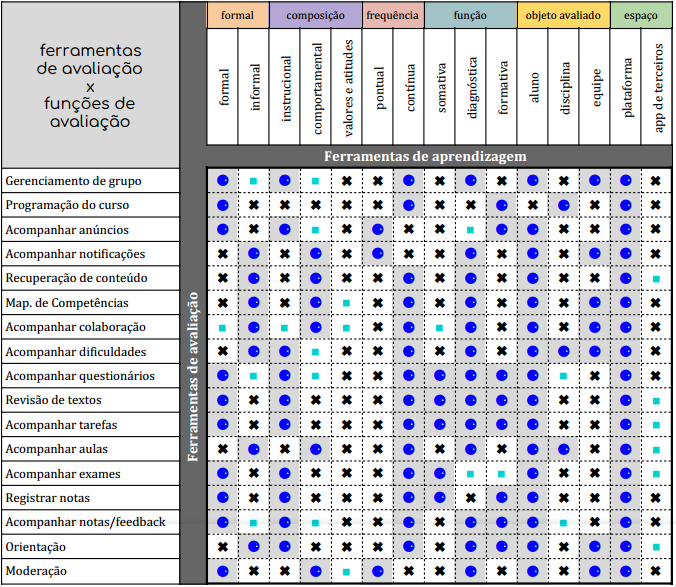
\includegraphics[width=\textwidth]{img/avaliacao_funcoes.png}
%    \caption{Relação entre ferramentas de avaliação e funções de avaliação.}
%    \label{fig:funcoes}
%\end{figure}